\documentclass[12pt]{article}
\usepackage{amssymb}
\usepackage{amsmath}
\usepackage{commath}
\usepackage{amsthm}
\usepackage{graphicx}
\usepackage{hyperref}
\usepackage{subcaption}
\usepackage[section]{placeins}
\usepackage[margin=1in]{geometry}
\newcommand{\Z}{\mathbb{Z}}
\newcommand{\N}{\mathbb{N}}
\newcommand{\C}{\mathbb{C}}
\newcommand{\Q}{\mathbb{Q}}
\newcommand{\R}{\mathbb{R}}
\renewcommand{\thesubsection}{\alph{subsection}.}
\DeclareMathOperator{\dist}{dist}
\DeclareMathOperator{\avg}{avg}
%opening
\title{ML Final Project}
\author{Victor Zeng, Universon Van, Brenda Gonzalez, Youssef Mroue}
\counterwithin*{equation}{section}
\counterwithin*{equation}{subsection}

\hypersetup{
	colorlinks   = true, %Colours links instead of ugly boxes
	urlcolor     = blue, %Colour for external hyperlinks
	linkcolor    = blue, %Colour of internal links
	citecolor   = red %Colour of citations
}


\makeatletter
\newcommand{\chapterauthor}[1]{%
	{\parindent0pt\vspace*{-10pt}%
		\linespread{1.1}\large\scshape#1%
		\par\nobreak\vspace*{10pt}}
	\@afterheading%
}
\makeatother

\begin{document}

\maketitle
\newtheorem*{claim}{Claim:}
\newtheorem*{lemma}{Lemma}

\section{Introduction}
\chapterauthor{Victor Zeng}

One of the most frequent reasons people have cited for not voting is that "both parties are the same." At its core, this argument claims that one's vote does not matter because no matter which party gets elected, the resulting policies will be the same. 
In our analysis, we attempt to determine whether or not there is any merit to this claim. In particular, we want to answer the following question: 
\begin{center}
	Does the party affiliation of a politician predict how the politician will vote?  
\end{center}

To answer this question, we analyzed the 2012 House of Representatives roll call voting record, which we scraped  from the congressional bulk data site using the Congress data downloader tool  (\url{https://github.com/unitedstates/congress}). The data set consists of 435 observations (one row for each representative) of 659 variables. The variables include name, party (D/R), and their vote in each of the 657 roll call votes of the session by the representative for different issues (Yay (Y), Nay (N), Present (P), and Not Voting (O)).

Because we do not have any categories (i.e as conservative, libertarian, progressive, etc) for voting behavior, we must first find natural groupings in the voting behavior of representatives. This is a task naturally geared towards unsupervised learning. Once we have these natural groupings, we can then analyze the clusters to determine the answer to our question.
\section{Models}
\chapterauthor{Victor Zeng}
In our analysis, we will use the  Hierarchical and K-means clustering algorithms. Each one of these algorithms has their own set of advantages and disadvantages. K-means is computationally faster and tends to produce tighter clusters while hierarchical clustering is fully deterministic and only requires us to compute the dendrogram once for multiple Ks. 
\subsection{Hierarchical Clustering}
\chapterauthor{Brenda Gonzalez}
Hierarchical Clustering is a bottom-up clustering algorithm. It starts out with each observation in its own cluster and repeatedly merges the two most similar clusters. In our analysis, we used three different methods for calculating the similarity of the clusters: complete linkage, which is defined by 
$$D(X,Y) = \max_{x\in X,y\in Y} \dist(x,y),$$
\noindent
average linkage, which is defined by 
$$D(X,Y) = \frac{1}{\abs{X}\abs{Y}} \sum_{x\in X}\sum_{y\in Y} \dist(x,y),$$
and single linkage, which is defined by 
$$D(X,Y) = \min_{x\in X,y\in Y} \dist(x,y)$$
where $\dist(x,y)$ is the euclidean distance between the two points. 
\subsection{K-Means Clustering}
\chapterauthor{Brenda Gonzalez}
K-means is a clustering algorithm which partitions observations into a predetermined number of clusters. In particular, it attempts to find a clustering such that the within-cluster sum of squares distances is at a minimum. Formally speaking, it seeks to find
$$\arg \min_{S}\sum_{i=1}^{k}\sum_{x\in S_i}\norm{x-c}^2$$
It does so by randomly assigning each observation to one of K clusters. We then repeatedly compute the cluster centroid 
$$c_i = \frac{1}{\abs{X}}\sum_{x\in X}x_i$$
and reassign each observation to the cluster whose centroid is the closest. This process repeats itself until the clusters no longer change. 

Because this iterative process only finds a local minima, the final clusters depend heavily on the results of the initial random clustering. We are not guaranteed that the final clusters will be the global optima. As such, the algorithm is normally run multiple times with different random initial random clustering and the best final clusters are chosen. 
\subsection{Model Fitting Considerations}
\chapterauthor{Youssef Mroue}
In order to apply either model, we needed the data/votes of each representative to be numerical rather than four different string values. In order to differentiate between the different type of votes, we converted the "Yay" votes to 1, the "Nay" votes to -1, and the "Present" and "Not Voting" votes to 0. Because we wished to determine similarity solely based on the voting record,  we excluded the name, party, ID \#, and state predictors from the data we clustered. In addition, because they do not convey any useful information, we also removed the roll call votes which were completely unanimous. There was no need to scale the data since the variables we used were in the same scale (0, 1, and -1). 

\section{Analysis}
\subsection{Hierarchical Clustering}
\chapterauthor{Universon Van,Youssef Mroue,Brenda Gonzalez}
We start out by using the silhouette coefficients to determine the optimal K for each linkage method. In this analysis, we found that k = 4 for single linkage, and k = 2 for both complete and average linkage. 
\begin{figure}[h]
	\caption{Optimal K by linkage method}
	\begin{subfigure}{0.45\textwidth}
		\caption{Single Linkage}		
		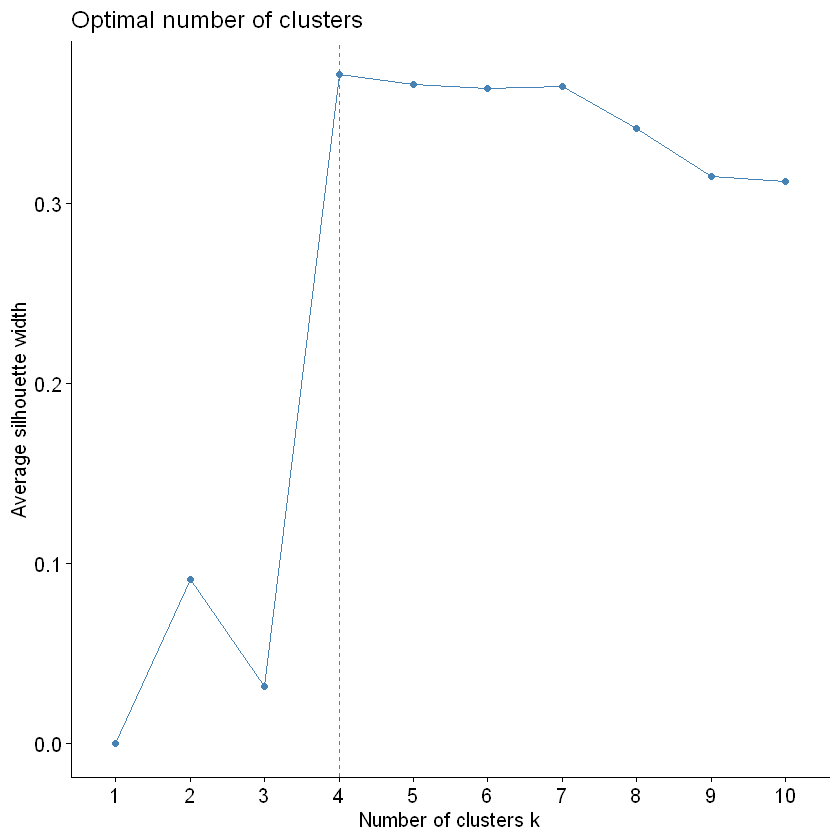
\includegraphics[width=\textwidth]{Images/Hierarchial_silhouette_single}
	\end{subfigure}
	\centering
	\begin{subfigure}{0.45\textwidth}
		\caption{Complete Linkage}
		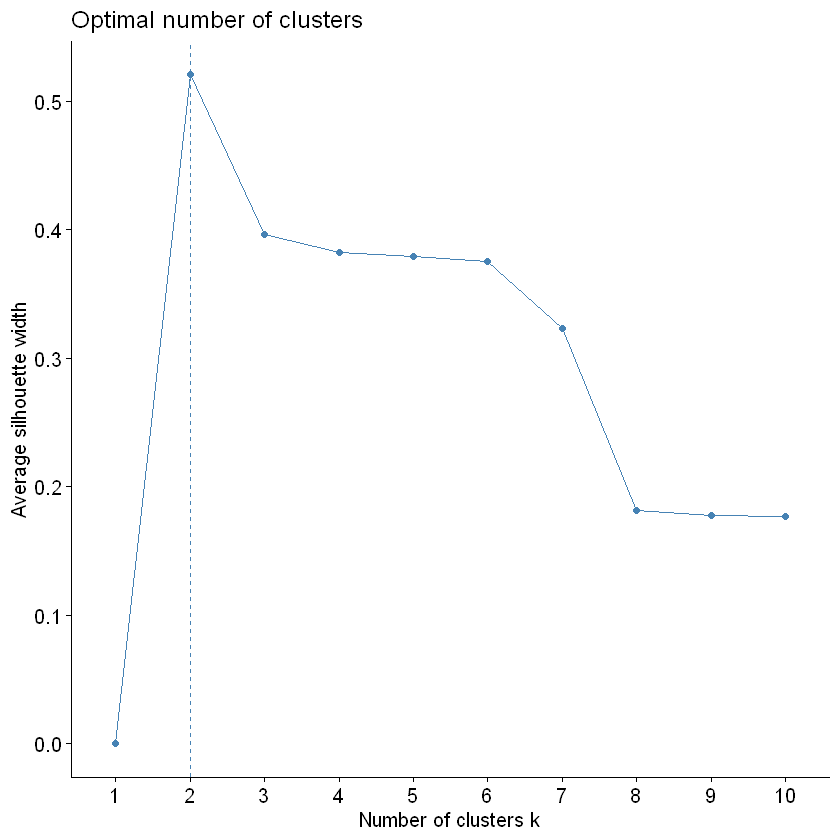
\includegraphics[width=\textwidth]{Images/Hierarchial_silhouette_complete}
	\end{subfigure}
	\begin{subfigure}{0.45\textwidth}
		\caption{Average Linkage}		
		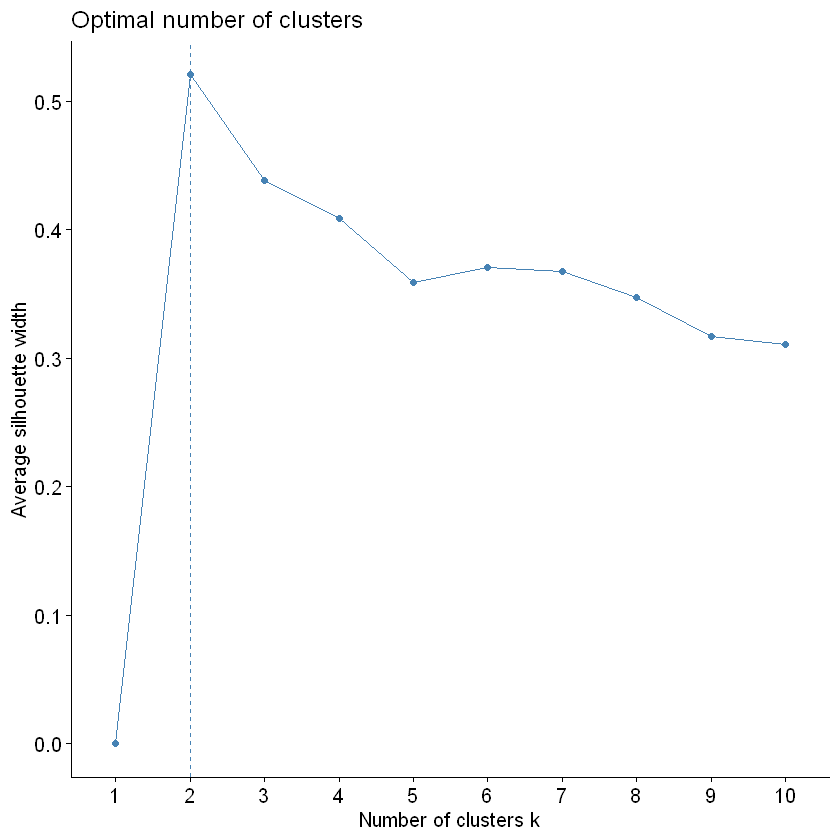
\includegraphics[width=\textwidth]{Images/Hierarchial_silhouette_average}
	\end{subfigure}
\end{figure}
We then compared the silhouette values for the optimal k of each linkage and found that complete and average linkage tied for highest silhouette values. 
\begin{table}[h]
	\caption{Silhouette coefficient of optimal Ks}
	\centering
	\begin{tabular}{r|r}
		Linkage Method & Optimal Silhouette Coefficient \\
		\hline
		Single & 0.3713787 \\
		Average & 0.5208278 \\
		Complete & 0.5208278
	\end{tabular}
\end{table}

Because they tied for the highest silhouette coefficient, we decided to use both average and complete linkage with a $k$ of 2. Upon generating the clusters, we found that both complete linkage and single linkage produced the same clusters. We believe that this is strong evidence that the clusters are indeed valid clustering. Likewise, looking at the dendrograms for the two groups, we can see that there are two clearly distinct groups in the data set. 
\begin{figure}[h]
	\caption{Hierarchical clustering dendograms}
	\begin{subfigure}{0.45\textwidth}	
		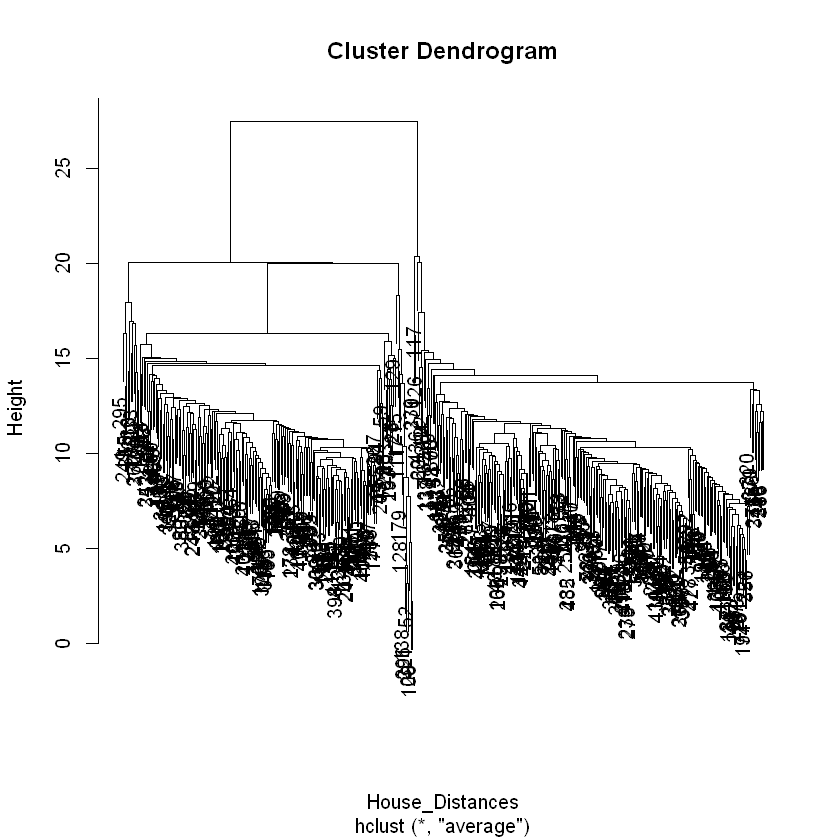
\includegraphics[width=\textwidth]{Images/dendogram_average}
	\end{subfigure}
	\centering
	\begin{subfigure}{0.45\textwidth}
		
		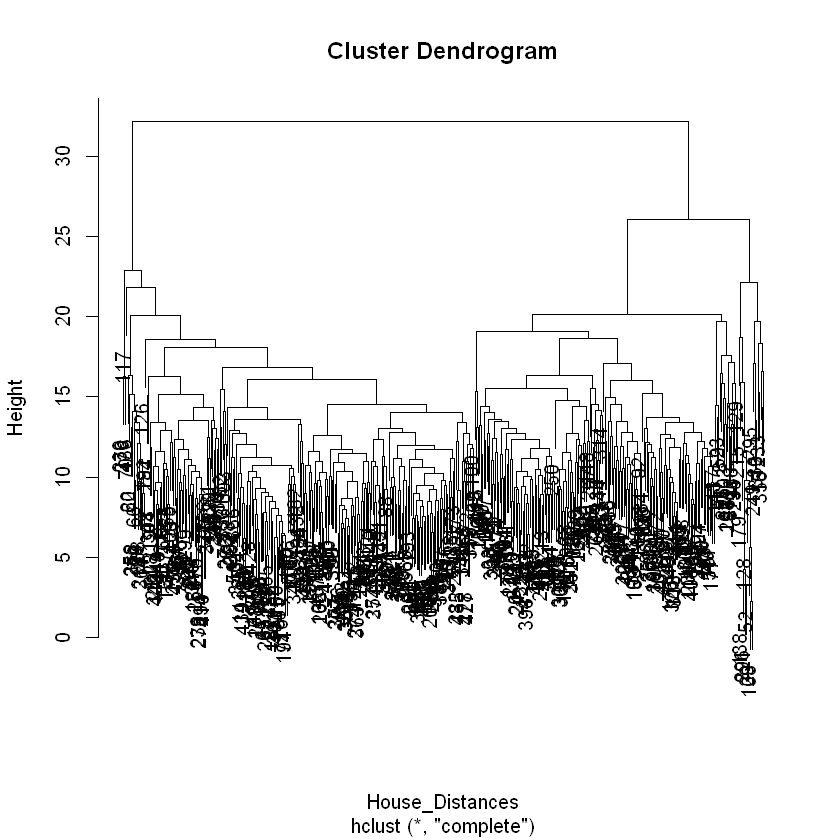
\includegraphics[width=\textwidth]{Images/dendogram_complete}
	\end{subfigure}
\end{figure}

We then proceeded to look at the party composition of the two clusters. 
\begin{table}[h]
	\caption{Party Composition of the Hierarchical Clusters}
	\centering
	\begin{tabular}{l|ll}
		& D & R \\
		\hline
		Cluster 1 & 197 & 2 \\
		Cluster 2 & 0 & 241
	\end{tabular}
\end{table}
As expected, the clusters were split almost perfectly along party lines, indicating that the parties are very different. However, we found that two Republicans, John Boehner and Thomas Massie, were placed in the Democrat cluster rather than the Republican cluster. We will call any misclassified representatives as traitors as the clustering shows that they vote more similar to the opposite party than their own. 
\FloatBarrier
\subsection{K-Means}
\chapterauthor{Universon Van,Youssef Mroue}
To verify this finding, we then proceeded to run the same analysis with K-means. Using the elbow method, we found that there was an optimal $k$ of 2. 
\begin{figure}[h]
	\caption{Total WSS (Elbow Method)}
	\centering
	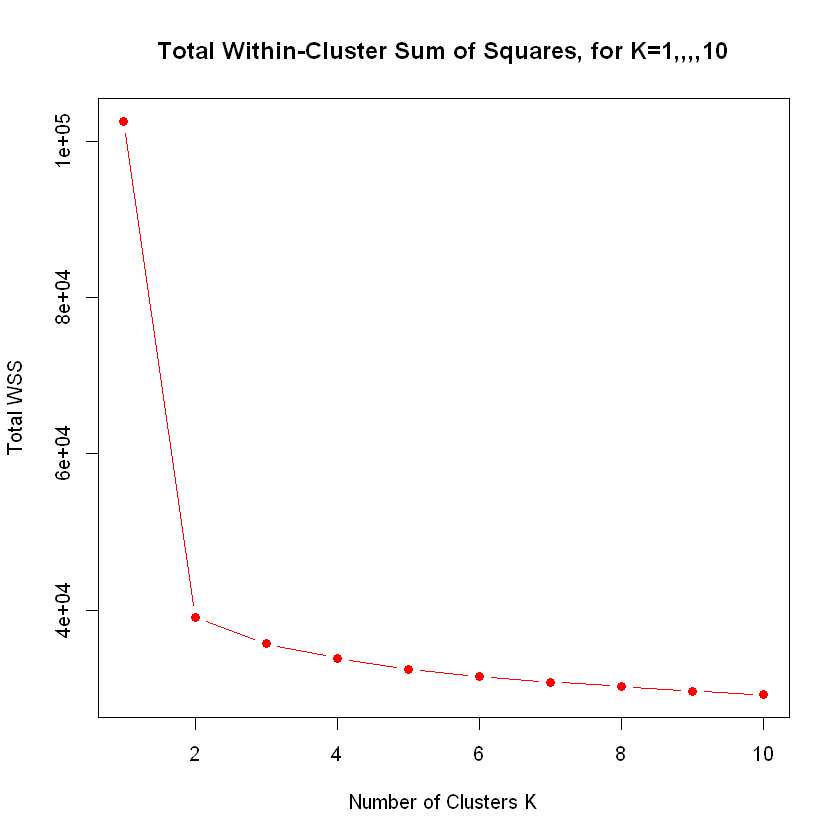
\includegraphics[width=.5\textwidth]{Images/Elbow}
\end{figure}
The resulting clustering had a slightly higher silhouette coefficient of 0.52358, and was similarly partisan. However, unlike the Hierarchical model, it produced one Republican and three Democratic traitors, John Boehner, Boren, Shuler, Matheson. Of these, only Boehner was named a traitor by both clustering methods, suggesting that the others were statistical anomalies.  
\begin{table}[h]
	\caption{Party Composition of the K-Means Clusters}
	\centering
	\begin{tabular}{l|ll}
		& D & R \\
		\hline
		Cluster 1 & 194 & 1 \\
		Cluster 2 & 3 & 242
	\end{tabular}
\end{table}
\section{Model Comparison}
\chapterauthor{Universon Van}
While K-means had a slightly better silhouette coefficient than any of the hierarchical clustering linkages we tried, the difference of 0.00276 is fairly negligible. As such, we still prefer hierarchical due to its deterministic nature and its lower computational cost. Moreover, in the hierarchical model, we can easily see whether there are any further sub-factions within the two parties by looking at the dendrogram. 
\begin{figure}[h]
	\centering
	\begin{subfigure}{.45\linewidth}
		\caption{K-means clusters}		
		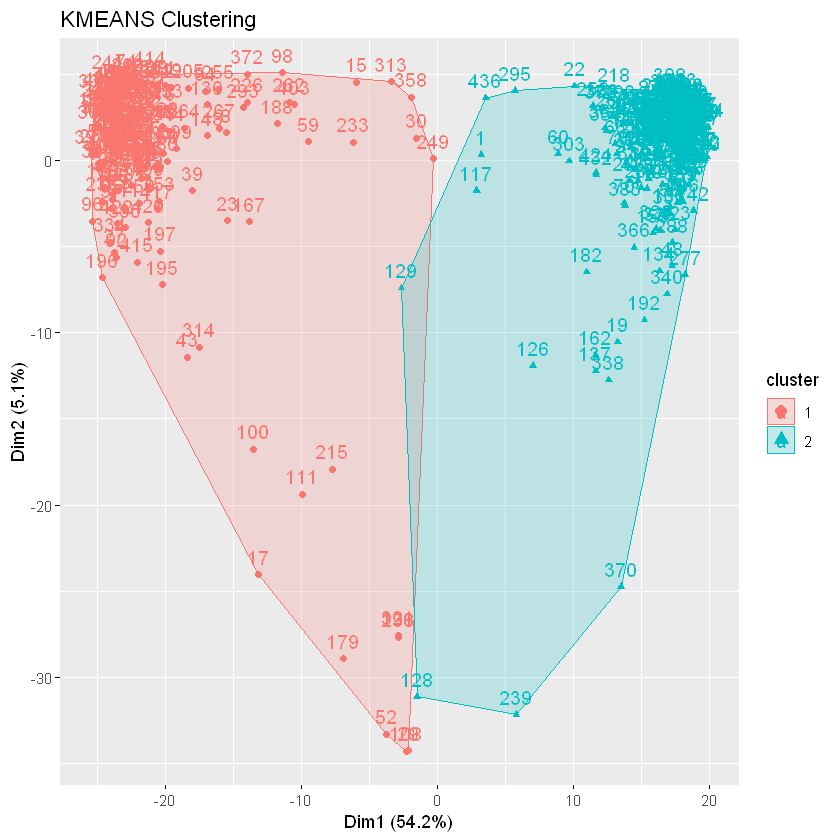
\includegraphics[width=\textwidth]{Images/kmeans_cluster}
	\end{subfigure}
	\begin{subfigure}{.45\linewidth}
		\caption{Hierarchical clusters}		
		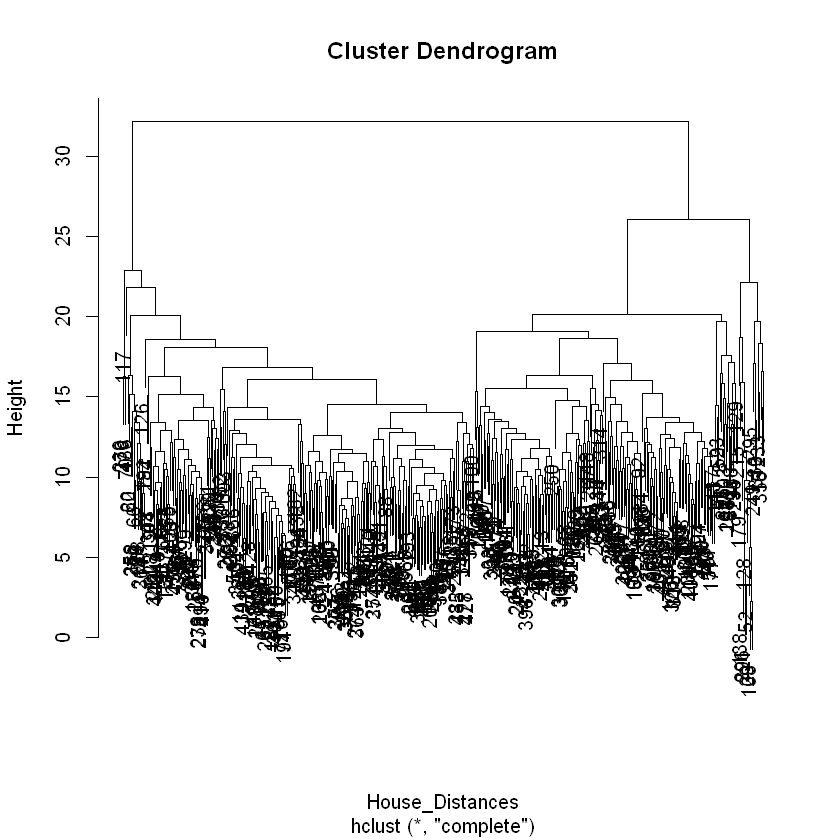
\includegraphics[width=\textwidth]{Images/dendogram_complete}
	\end{subfigure}
\end{figure}  
\section{Conclusion}
\chapterauthor{Victor Zeng}
In our analysis, we found strong evidence that the common allegation that "both parties are the same" is incorrect. If such a claim were true, then the party affiliation of a politician would have little to no predictive value on their voting record, and as such we would expect that when clustering only on the voting record of representatives, the resulting clusters would be very bipartisan with a roughly equal ratio of democrats to republicans. However, both clustering models produced clusters which were for all intents and purposes split along party lines.  

With each model, only a few ($<5$) representatives were placed in a cluster with the opposing party. These representatives, which we call party traitors, were predominately centralists who were known for voting across the aisle. Of special note, however, is the single representative who was identified as a party traitor by both models, John Boehner. In 2014, two years after the votes in our dataset, he retired from Congress due to personal disagreements with the direction of the GOP.

\end{document}
